\documentclass[12pt]{article}
\everymath{\displaystyle}
\usepackage{unicode-math}
\usepackage{pgfplots}
\pgfplotsset{compat=1.18}
\usepackage{amsmath}



\usepackage[margin=1in]{geometry}
\usepackage{tcolorbox}
\usepackage{graphicx}
\usepackage{tikz}
\usepackage{amssymb}
\usepackage{enumitem}
\usepackage{titlesec}
\usepackage{fancyhdr}
\usepackage{pifont}
\usepackage{xcolor}
\newcounter{questionnum}
\setcounter{questionnum}{0}
\usepackage{eso-pic} % for page background

% --------- 主题颜色设置 ---------
\definecolor{novelblue}{RGB}{70,60,150}
\definecolor{headerbg}{RGB}{240,240,255}

\pagestyle{fancy}
\fancyhf{}
\renewcommand{\headrulewidth}{0.4pt}
\renewcommand{\headrule}{\hbox to\headwidth{\color{novelblue}\leaders\hrule height 0.4pt\hfill}}

% --------- 页眉背景色条 ---------
\newcommand{\headbackground}{
  \AddToShipoutPictureBG*{
    \begin{tikzpicture}[remember picture, overlay]
      \fill[blue!5!purple!10] (current page.north west) rectangle ([yshift=-60pt]current page.north east);
    \end{tikzpicture}
  }
}

% --------- 页眉设置 ---------
\pagestyle{fancy}
\fancyhf{}
\renewcommand{\headrulewidth}{0pt}
\fancyhead[L]{\color{novelblue}\textbf{\textbf{Novel Prep} }}
\fancyhead[C]{\color{novelblue}\textbf {SAT Preparation}}
\fancyhead[R]{\color{novelblue}\textbf{Jack Zeng}}


\newtcolorbox{SATCard}[1][]{%
  enhanced,
  colback=white,
  colframe=novelblue,
  coltitle=white,
  boxrule=0.6pt,
  arc=4pt,
  boxsep=5pt,
  left=8pt, right=8pt, top=10pt, bottom=10pt,
  sharp corners=south,
  drop shadow south east,
  #1
}

% --------- 顶部 Mark for Review 栏 ---------
\newcommand{\markforreview}{
  \stepcounter{questionnum} % 自动递增题号
  \begin{tikzpicture}[scale=1.1]
    % 黑色题号
    \fill[black] (0,0) rectangle (0.8,0.6);
    \node[white, font=\bfseries\large] at (0.4,0.3) {\thequestionnum};

    % 灰底主栏
    \fill[gray!10] (0.8,0) rectangle (14.5,0.6);

    % Mark for Review
    \node[anchor=west, font=\small] at (1.2,0.3) {\ding{72} \hspace{2pt}Mark for Review};

    % ABC 按钮区域
    \draw[thick, rounded corners=3pt] (13.5,0.12) rectangle (14.5,0.48);
    \node[font=\bfseries\normalsize] at (14.0,0.3) {ABC};
  \end{tikzpicture}


  \newcommand{\choiceboxcircled}[2]{%
  \begin{tcolorbox}[
    colback=white,
    colframe=black,
    boxrule=0.5pt,
    rounded corners=6pt,
    left=6pt, right=6pt, top=6pt, bottom=6pt,
    width=\linewidth
  ]
    \textbf{\large\textcircled{\textbf{#1}}} \ #2
  \end{tcolorbox}
}
}

% --------- 选项框样式 ---------
\newcommand{\choicebox}[2]{%
  \begin{tcolorbox}[
    colback=white, 
    colframe=novelblue,
    boxrule=0.5pt, 
    rounded corners=4pt, 
    left=6pt, right=6pt, top=6pt, bottom=6pt,
    width=\linewidth
  ]
  \textbf{#1.} \ #2
  \end{tcolorbox}
}


\begin{document}


\section*{Math Hard Question 3}



\noindent\markforreview
\vspace{1em}

A research manager selected 2 random samples of ovens of a certain type to estimate the average amount of time this type of oven takes to preheat to \(325^\circ F\).  
The research manager recorded the amount of time, in minutes, each oven takes to preheat to \(325^\circ F\).

Based on the first sample, the manager estimated an average of 14.2 minutes, with a margin of error of 1 minute.  
Based on the second sample, the estimate was 14.4 minutes, with a margin of error of 2.3 minutes.

Assuming the margins of error were calculated the same way, which of the following best explains why the first sample had a smaller margin of error?

\vspace{0.75em}

\choicebox{A}{The first sample contained fewer ovens than the second sample.}  
\choicebox{B}{The first sample contained more ovens than the second sample.}  
\choicebox{C}{The first sample took less time on average to preheat.}  
\choicebox{D}{The first sample took more time on average to preheat.}

\vspace{2em}
\newpage
\noindent\markforreview
\vspace{1em}

\begin{center}
    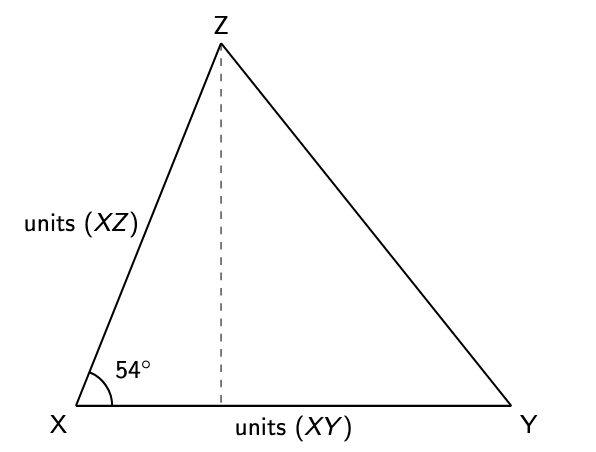
\includegraphics[width=0.45\linewidth]{f9.png}
\end{center}

In triangle \(XYZ\), \(\angle X = 54^\circ\), \(XY = 26\) units, \(XZ = 19\) units.  
What is the area, in square units, of triangle \(XYZ\)?

\vspace{0.75em}

\choicebox{A}{247}  
\choicebox{B}{494}  
\choicebox{C}{247\sin 54^\circ}  
\choicebox{D}{494\sin 54^\circ}

\vspace{2em}







\vspace{2em}
\noindent\markforreview
\vspace{1em}

In the figure, \(\triangle ABC\) is inscribed in a semicircle with diameter \(AC = 10\).  
Point \(B\) lies on the semicircle. If \(AB = 6\) and \(BC = x\), find \(x\).  
Give your answer in simplest radical form.

\vspace{0.75em}

\choicebox{A}{\(\sqrt{36}\)}  
\choicebox{B}{8}  
\choicebox{C}{\(\sqrt{44}\)}  
\choicebox{D}{\(\sqrt{64}\)}

\vspace{2em}

\noindent\markforreview
\vspace{1em}

A parabola is given by  
\[
y = x^2 - 4x + 5,
\]
and a circle by  
\[
x^2 + y^2 = 25.
\]

The parabola and circle intersect at points \(P\) and \(Q\).  
Find the distance between \(P\) and \(Q\).



\newpage
\noindent\markforreview
\vspace{1em}

Solve the equation:  
\[
\sqrt{6r} = \sqrt{r^2 - 16}
\]

What is the product of all solutions to the above equation?

\vspace{0.75em}

\choicebox{A}{4}  
\choicebox{B}{6}  
\choicebox{C}{8}  
\choicebox{D}{12}



\end{document}